\documentclass[9pt]{beamer}
\usepackage[utf8]{inputenc}
\usepackage{adjustbox}
\usepackage{amsmath,amssymb,amsthm}
\usepackage{cancel}
\usepackage{float}
\usepackage{mathtools}
\usepackage{dsfont}
\usepackage{tcolorbox}
\usepackage{texdraw}
\usepackage{tikz}
\usepackage{todonotes}
\usepackage{pgfplots}

\usetikzlibrary{arrows}

\usepgfplotslibrary{fillbetween}

\pgfplotsset{compat=1.16}

\usetheme{Warsaw}

\makeatletter
\setbeamertemplate{footline}
{
    \leavevmode%
    \hbox{%
    \begin{beamercolorbox}[wd=.5\paperwidth,ht=2.5ex,dp=2ex,center]{title in head/foot}%
        \usebeamerfont{title in head/foot}\vspace{-3pt}{\footnotesize Diamond Duplication Glitch}
    \end{beamercolorbox}%
    \begin{beamercolorbox}[wd=.5\paperwidth,ht=2.5ex,dp=2ex,right]{date in head/foot}%
        \usebeamerfont{name in head/foot}\vspace{-3pt}{\footnotesize \insertauthor{}\hspace*{6em}
        \insertframenumber{} / \inserttotalframenumber\hspace*{2ex}}
    \end{beamercolorbox}}%
    \vskip0pt%
}
\makeatother

\usetikzlibrary{arrows.meta}

\title{Diamond Duplication Glitch (Working 22/05/2025)}
\author{Alec Elhindi}
\date{22 May 2025}

\usepackage{graphicx}
\graphicspath{{./images/}}

\newcounter{definition}

\renewcommand{\definition}[1]{\vspace{6pt}\textbf{Definition~\refstepcounter{definition}\thedefinition}: \textit{#1}\vspace{6pt}}

\newcounter{conjecture}

\newcommand{\conjecture}[1]{\vspace{6pt}\textbf{Conjecture~\refstepcounter{conjecture}\theconjecture}: \textit{#1}\vspace{6pt}}

\renewcommand{\theorem}[1]{\vspace{6pt}\textbf{Theorem~\refstepcounter{theorem}\thetheorem}: \textit{#1}\vspace{6pt}}

\newcounter{proposition}

\newcommand{\proposition}[1]{\textbf{Proposition}: #1}

\renewcommand{\proof}[1]{\textbf{Proof}: #1\vspace{12pt}}

\newcommand{\notation}[1]{\textbf{Notation}: #1}

\renewcommand{\qedsymbol}{$\blacksquare$}

\DeclarePairedDelimiter\abs{\lvert}{\rvert}

\makeatletter
\newcommand{\vast}{\bBigg@{4}}
\newcommand{\Vast}{\bBigg@{5}}
\makeatother

\definecolor{electricpurple}{rgb}{0.75, 0.0, 1.0}

\newcommand{\red}[1]{{\color{red} #1}}
\newcommand{\blue}[1]{{\color{blue} #1}}
\newcommand{\orange}[1]{{\color{orange} #1}}
\newcommand{\purple}[1]{{\color{electricpurple} #1}}

\makeatletter
\let\save@measuring@true\measuring@true
\def\measuring@true{%
  \save@measuring@true
  \def\beamer@sortzero##1{\beamer@ifnextcharospec{\beamer@sortzeroread{##1}}{}}%
  \def\beamer@sortzeroread##1<##2>{}%
  \def\beamer@finalnospec{}%
}
\makeatother

\definecolor{violet}{rgb}{0.56, 0.0, 1.0}
\definecolor{indigo}{rgb}{0.29, 0.0, 0.51}

\begin{document}

    \begin{frame}

        \titlepage

    \end{frame}

    \begin{frame}{Riemann Integration}

        \begin{center}
        
            \begin{tikzpicture}[declare function={f(\x)=-(\x-2)^2+4;}]
    
                \begin{axis}[
                        axis x line=middle,
                        axis y line=middle,
                        axis line style={=>},
                        xmin=-1,xmax=5,
                        ymin=-1,ymax=5,
                        xlabel=$x$,
                        ylabel=$y$,
                        xtick=\empty,
                        ytick=\empty,
                        xticklabels=\empty,
                        yticklabels=\empty,
                    ]
                    \addplot[smooth, thick, black]{f(x)};
                    \draw (2, {f(2)}) node[above right]{$y=-(x-2)^2+4$};
                \end{axis}
                
            \end{tikzpicture}

        \end{center}

    \end{frame}

    \begin{frame}{Riemann Integration}

        \begin{center}
        
            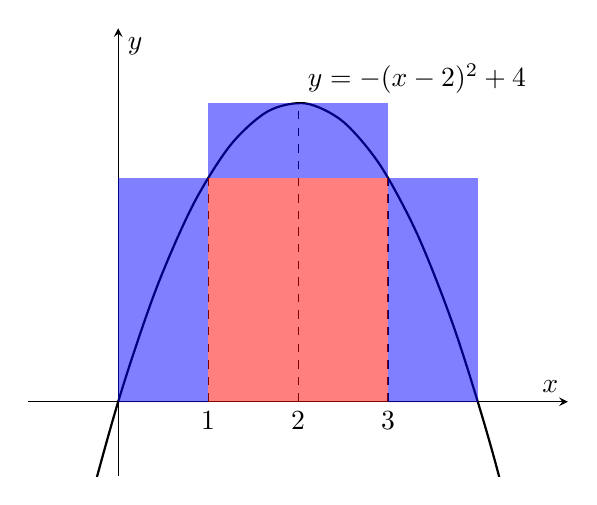
\begin{tikzpicture}[declare function={f(\x)=-(\x-2)^2+4;}]
    
                \begin{axis}[
                        axis x line=middle,
                        axis y line=middle,
                        axis line style={=>},
                        xmin=-1,xmax=5,
                        ymin=-1,ymax=5,
                        xlabel=$x$,
                        ylabel=$y$,
                        xtick=\empty,
                        ytick=\empty,
                        xticklabels=\empty,
                        yticklabels=\empty,
                    ]
                    \addplot[smooth, thick, black]{f(x)};
                    \draw[dashed] (1, 0) node[below]{$1$}-- (1, {f(1)});
                    \draw[dashed] (2, 0) node[below]{$2$}-- (2, {f(2)}) node[above right]{$y=-(x-2)^2+4$};
                    \draw[dashed] (3, 0) node[below]{$3$}-- (3, {f(3)});
                    
                    \path[fill=blue, opacity=0.5] (0, 0) -- (1, 0) -- (1, {f(1)}) -- (0, {f(1)});
                    \path[fill=red, opacity=0.5] (0, 0) -- (1, 0) -- (1, {f(0)}) -- (0, {f(0)});
                    \path[fill=blue, opacity=0.5] (1, f{(1)}) -- (2, {f(1)}) -- (2, {f(2)}) -- (1, {f(2)});
                    \path[fill=red, opacity=0.5] (1, 0) -- (2, 0) -- (2, {f(1)}) -- (1, {f(1)});
                    
                    \path[fill=blue, opacity=0.5] (2, f{(2)}) -- (3, {f(2)}) -- (3, {f(3)}) -- (2, {f(3)});
                    \path[fill=red, opacity=0.5] (2, 0) -- (3, 0) -- (3, {f(3)}) -- (2, {f(3)});
                    \path[fill=blue, opacity=0.5] (3, f{(3)}) -- (4, {f(3)}) -- (4, {f(4)}) -- (3, {f(4)});
                    \path[fill=red, opacity=0.5] (3, 0) -- (4, 0) -- (4, {f(4)}) -- (3, {f(4)});
                \end{axis}
                
            \end{tikzpicture}

        \end{center}

    \end{frame}

    \begin{frame}{Riemann Integration}

        \begin{center}
        
            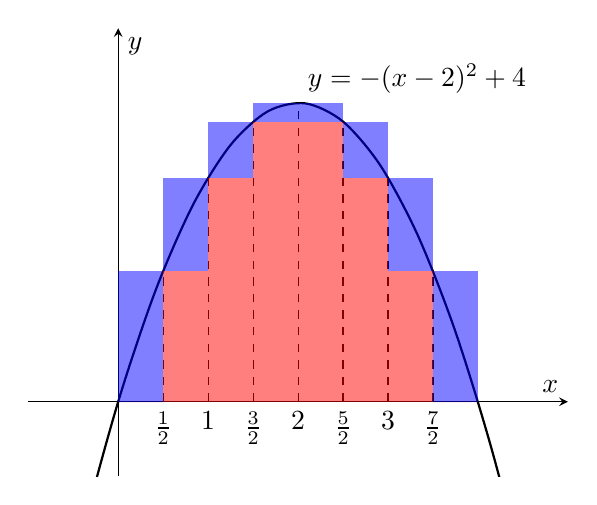
\begin{tikzpicture}[declare function={f(\x)=-(\x-2)^2+4;}]
    
                \begin{axis}[
                        axis x line=middle,
                        axis y line=middle,
                        axis line style={=>},
                        xmin=-1,xmax=5,
                        ymin=-1,ymax=5,
                        xlabel=$x$,
                        ylabel=$y$,
                        xtick=\empty,
                        ytick=\empty,
                        xticklabels=\empty,
                        yticklabels=\empty,
                    ]
                    \addplot[smooth, thick, black]{f(x)};
                    \draw[dashed] (0.5, 0) node[below]{$\frac{1}{2}$}-- (0.5, {f(0.5)});
                    \draw[dashed] (1, 0) node[below]{$1$}-- (1, {f(1)});
                    \draw[dashed] (1.5, 0) node[below]{$\frac{3}{2}$}-- (1.5, {f(1.5)});
                    \draw[dashed] (2, 0) node[below]{$2$}-- (2, {f(2)}) node[above right]{$y=-(x-2)^2+4$};
                    \draw[dashed] (2.5, 0) node[below]{$\frac{5}{2}$}-- (2.5, {f(2.5)});
                    \draw[dashed] (3, 0) node[below]{$3$}-- (3, {f(3)});
                    \draw[dashed] (3.5, 0) node[below]{$\frac{7}{2}$}-- (3.5, {f(3.5)});
                    
                    \path[fill=blue, opacity=0.5] (0, 0) -- (0.5, 0) -- (0.5, {f(0.5)}) -- (0, {f(0.5)});
                    \path[fill=red, opacity=0.5] (0, 0) -- (0.5, 0) -- (0.5, {f(0)}) -- (0, {f(0)});
                    \path[fill=blue, opacity=0.5] (0.5, {f(0.5)}) -- (1, {f(0.5)}) -- (1, {f(1)}) -- (0.5, {f(1)});
                    \path[fill=red, opacity=0.5] (0.5, 0) -- (1, 0) -- (1, {f(0.5)}) -- (0.5, {f(0.5)});
                    \path[fill=blue, opacity=0.5] (1, {f(1)}) -- (1.5, {f(1)}) -- (1.5, {f(1.5)}) -- (1, {f(1.5)});
                    \path[fill=red, opacity=0.5] (1, 0) -- (1.5, 0) -- (1.5, {f(1)}) -- (1, {f(1)});
                    \path[fill=blue, opacity=0.5] (1.5, {f(1.5)}) -- (2, {f(1.5)}) -- (2, {f(2)}) -- (1.5, {f(2)});
                    \path[fill=red, opacity=0.5] (1.5, 0) -- (2, 0) -- (2, {f(1.5)}) -- (1.5, {f(1.5)});
                    
                    \path[fill=blue, opacity=0.5] (2, f{(2)}) -- (2.5, {f(2)}) -- (2.5, {f(2.5)}) -- (2, {f(2.5)});
                    \path[fill=red, opacity=0.5] (2, 0) -- (2.5, 0) -- (2.5, {f(2.5)}) -- (2, {f(2.5)});
                    \path[fill=blue, opacity=0.5] (2.5, f{(2.5)}) -- (3, {f(2.5)}) -- (3, {f(3)}) -- (2.5, {f(3)});
                    \path[fill=red, opacity=0.5] (2.5, 0) -- (3, 0) -- (3, {f(3)}) -- (2.5, {f(3)});
                    \path[fill=blue, opacity=0.5] (3, f{(3)}) -- (3.5, {f(3)}) -- (3.5, {f(3.5)}) -- (3, {f(3.5)});
                    \path[fill=red, opacity=0.5] (3, 0) -- (3.5, 0) -- (3.5, {f(3.5)}) -- (3, {f(3.5)});
                    \path[fill=blue, opacity=0.5] (3.5, f{(3.5)}) -- (4, {f(3.5)}) -- (4, {f(4)}) -- (3.5, {f(4)});
                    \path[fill=red, opacity=0.5] (3.5, 0) -- (4, 0) -- (4, {f(4)}) -- (3.5, {f(4)});
                \end{axis}
                
            \end{tikzpicture}

        \end{center}

    \end{frame}

    \begin{frame}{Riemann Integration}

        \begin{center}
        
            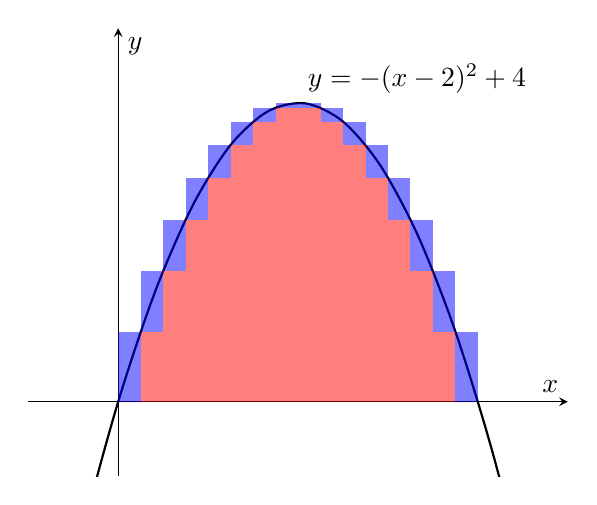
\begin{tikzpicture}[declare function={f(\x)=-(\x-2)^2+4;}]
    
                \begin{axis}[
                        axis x line=middle,
                        axis y line=middle,
                        axis line style={=>},
                        xmin=-1,xmax=5,
                        ymin=-1,ymax=5,
                        xlabel=$x$,
                        ylabel=$y$,
                        xtick=\empty,
                        ytick=\empty,
                        xticklabels=\empty,
                        yticklabels=\empty,
                    ]
                    \addplot[smooth, thick, black]{f(x)};
                    \draw (2, {f(2)}) node[above right]{$y=-(x-2)^2+4$};
                    
                    \path[fill=blue, opacity=0.5] (0, 0) -- (0.25, 0) -- (0.25, {f(0.25)}) -- (0, {f(0.25)});
                    \path[fill=red, opacity=0.5] (0, 0) -- (0.25, 0) -- (0.25, {f(0)}) -- (0, {f(0)});
                    \path[fill=blue, opacity=0.5] (0.25, {f(0.25)}) -- (0.5, {f(0.25)}) -- (0.5, {f(0.5)}) -- (0.25, {f(0.5)});
                    \path[fill=red, opacity=0.5] (0.25, 0) -- (0.5, 0) -- (0.5, {f(0.25)}) -- (0.25, {f(0.25)});
                    \path[fill=blue, opacity=0.5] (0.5, {f(0.5)}) -- (0.75, {f(0.5)}) -- (0.75, {f(0.75)}) -- (0.5, {f(0.75)});
                    \path[fill=red, opacity=0.5] (0.5, 0) -- (0.75, 0) -- (0.75, {f(0.5)}) -- (0.5, {f(0.5)});
                    \path[fill=blue, opacity=0.5] (0.75, {f(0.75)}) -- (1, {f(0.75)}) -- (1, {f(1)}) -- (0.75, {f(1)});
                    \path[fill=red, opacity=0.5] (0.75, 0) -- (1, 0) -- (1, {f(0.75)}) -- (0.75, {f(0.75)});
                    \path[fill=blue, opacity=0.5] (1, {f(1)}) -- (1.25, {f(1)}) -- (1.25, {f(1.25)}) -- (1, {f(1.25)});
                    \path[fill=red, opacity=0.5] (1, 0) -- (1.25, 0) -- (1.25, {f(1)}) -- (1, {f(1)});
                    \path[fill=blue, opacity=0.5] (1.25, {f(1.25)}) -- (1.5, {f(1.25)}) -- (1.5, {f(1.5)}) -- (1.25, {f(1.5)});
                    \path[fill=red, opacity=0.5] (1.25, 0) -- (1.5, 0) -- (1.5, {f(1.25)}) -- (1.25, {f(1.25)});
                    \path[fill=blue, opacity=0.5] (1.5, {f(1.5)}) -- (1.75, {f(1.5)}) -- (1.75, {f(1.75)}) -- (1.5, {f(1.75)});
                    \path[fill=red, opacity=0.5] (1.5, 0) -- (1.75, 0) -- (1.75, {f(1.5)}) -- (1.5, {f(1.5)});
                    \path[fill=blue, opacity=0.5] (1.75, {f(1.75)}) -- (2, {f(1.75)}) -- (2, {f(2)}) -- (1.75, {f(2)});
                    \path[fill=red, opacity=0.5] (1.75, 0) -- (2, 0) -- (2, {f(1.75)}) -- (1.75, {f(1.75)});
                    
                    \path[fill=blue, opacity=0.5] (2, {(f(2)}) -- (2.25, {(f(2)}) -- (2.25, {f(2.25)}) -- (2, {f(2.25)});
                    \path[fill=red, opacity=0.5] (2, 0) -- (2.25, 0) -- (2.25, {f(2.25)}) -- (2, {f(2.25)});
                    \path[fill=blue, opacity=0.5] (2.25, {f(2.25)}) -- (2.5, {f(2.25)}) -- (2.5, {f(2.5)}) -- (2.25, {f(2.5)});
                    \path[fill=red, opacity=0.5] (2.25, 0) -- (2.5, 0) -- (2.5, {f(2.5)}) -- (2.25, {f(2.5)});
                    \path[fill=blue, opacity=0.5] (2.5, {f(2.5)}) -- (2.75, {f(2.5)}) -- (2.75, {f(2.75)}) -- (2.5, {f(2.75)});
                    \path[fill=red, opacity=0.5] (2.5, 0) -- (2.75, 0) -- (2.75, {f(2.75)}) -- (2.5, {f(2.75)});
                    \path[fill=blue, opacity=0.5] (2.75, {f(2.75)}) -- (3, {f(2.75)}) -- (3, {f(3)}) -- (2.75, {f(3)});
                    \path[fill=red, opacity=0.5] (2.75, 0) -- (3, 0) -- (3, {f(3)}) -- (2.75, {f(3)});
                    \path[fill=blue, opacity=0.5] (3, {f(3)}) -- (3.25, {f(3)}) -- (3.25, {f(3.25)}) -- (3, {f(3.25)});
                    \path[fill=red, opacity=0.5] (3, 0) -- (3.25, 0) -- (3.25, {f(3.25)}) -- (3, {f(3.25)});
                    \path[fill=blue, opacity=0.5] (3.25, {f(3.25)}) -- (3.5, {f(3.25)}) -- (3.5, {f(3.5)}) -- (3.25, {f(3.5)});
                    \path[fill=red, opacity=0.5] (3.25, 0) -- (3.5, 0) -- (3.5, {f(3.5)}) -- (3.25, {f(3.5)});
                    \path[fill=blue, opacity=0.5] (3.5, {f(3.5)}) -- (3.75, {f(3.5)}) -- (3.75, {f(3.75)}) -- (3.5, {f(3.75)});
                    \path[fill=red, opacity=0.5] (3.5, 0) -- (3.75, 0) -- (3.75, {f(3.75)}) -- (3.5, {f(3.75)});
                    \path[fill=blue, opacity=0.5] (3.75, {f(3.75)}) -- (4, {f(3.75)}) -- (4, {f(4)}) -- (3.75, {f(4)});
                    \path[fill=red, opacity=0.5] (3.75, 0) -- (4, 0) -- (4, {f(4)}) -- (3.75, {f(4)});
                \end{axis}
                
            \end{tikzpicture}

        \end{center}

    \end{frame}

    \begin{frame}{What is Integration?}

        We can integrate `nice' functions.
        What about

        \[f(x)=1_\mathbb{Q}=\begin{cases}
            1\quad\text{if}\;x\in\mathbb{Q}\\
            0\quad\text{else}
        \end{cases}\]
        can we integrate this? \pause
        Naively one might say

        \[\int_{-\infty}^\infty 1_\mathbb{Q}\;dx\pause=\int_{-\infty}^\infty \sum_{a\in\mathbb{Q}} 1_a\pause=\sum_{a\in\mathbb{Q}}\int_{-\infty}^\infty 1_a\pause=\sum_{a\in\mathbb{Q}} \int_a^a 1\;dx\pause=\sum_{a\in\mathbb{Q}} (a-a)=0.\]\pause
        Can we even do this?
        
    \end{frame}

    \begin{frame}{What is Integration?}
    
        \[\int_{-\infty}^\infty 1_\mathbb{Q}\;dx=\int_{-\infty}^\infty \sum_{a\in\mathbb{Q}} 1_a=\sum_{a\in\mathbb{Q}}\int_{-\infty}^\infty 1_a=\sum_{a\in\mathbb{Q}} \int_a^a 1\;dx=\sum_{a\in\mathbb{Q}} (a-a)=0.\]
        What about

        \[1_{\mathbb{R}\setminus\mathbb{Q}}=\begin{cases}
            0\quad\text{if}\;x\in\mathbb{Q}\\
            1\quad\text{else}
        \end{cases}\]
        is the integral of this also $0$?\pause

        \[\int_{-\infty}^\infty 1_{\mathbb{R}\setminus\mathbb{Q}}\;dx=\int_{-\infty}^\infty \sum_{a\in\mathbb{R}\setminus\mathbb{Q}} 1_a=\sum_{a\in\mathbb{R}\setminus\mathbb{Q}}\int_{-\infty}^\infty 1_a=\sum_{a\in\mathbb{R}\setminus\mathbb{Q}} \int_a^a 1\;dx=\sum_{a\in\mathbb{R}\setminus\mathbb{Q}} (a-a)=0.\]\pause
        So

        \[\int_{-\infty}^\infty 1\;dx=\int_{-\infty}^\infty 1_\mathbb{Q}+1_{\mathbb{R}\setminus\mathbb{Q}}\;dx=\int_{-\infty}^\infty 1_\mathbb{Q}\;dx+\int_{-\infty}^\infty 1_{\mathbb{R}\setminus\mathbb{Q}}\;dx=0\]
        something is wrong...

    \end{frame}

    \begin{frame}{What is Integration?}

        \pause

        Using Reimann integration, we are assigning the set

        \[\{(x, y)\in\mathbb{R}^2\;|\;0\leq y\leq f(x)\;\text{or}\;f(x)\leq y\leq 0, x\in S\}\]
        a volume of
        
        \[\int_S f(x)\;dx.\]\pause
        Lebesgue wanted to know: can we assign a notion of volume to \textbf{all sets}?

    \end{frame}

    \begin{frame}{Riemann Integration}

        \begin{center}
        
            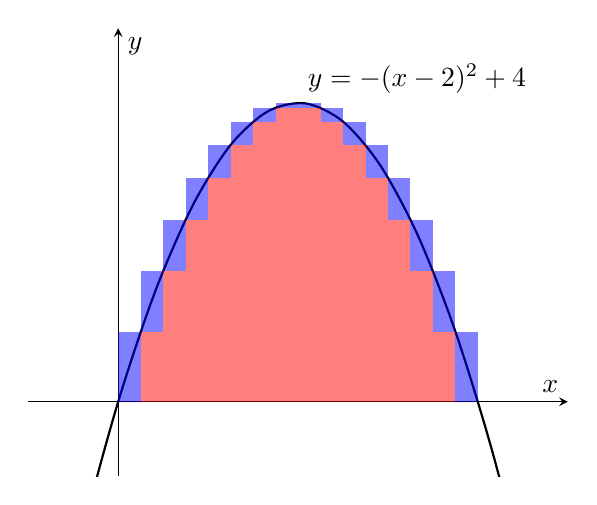
\begin{tikzpicture}[declare function={f(\x)=-(\x-2)^2+4;}]
    
                \begin{axis}[
                        axis x line=middle,
                        axis y line=middle,
                        axis line style={=>},
                        xmin=-1,xmax=5,
                        ymin=-1,ymax=5,
                        xlabel=$x$,
                        ylabel=$y$,
                        xtick=\empty,
                        ytick=\empty,
                        xticklabels=\empty,
                        yticklabels=\empty,
                    ]
                    \addplot[smooth, thick, black]{f(x)};
                    \draw (2, {f(2)}) node[above right]{$y=-(x-2)^2+4$};
                    
                    \path[fill=blue, opacity=0.5] (0, 0) -- (0.25, 0) -- (0.25, {f(0.25)}) -- (0, {f(0.25)});
                    \path[fill=red, opacity=0.5] (0, 0) -- (0.25, 0) -- (0.25, {f(0)}) -- (0, {f(0)});
                    \path[fill=blue, opacity=0.5] (0.25, {f(0.25)}) -- (0.5, {f(0.25)}) -- (0.5, {f(0.5)}) -- (0.25, {f(0.5)});
                    \path[fill=red, opacity=0.5] (0.25, 0) -- (0.5, 0) -- (0.5, {f(0.25)}) -- (0.25, {f(0.25)});
                    \path[fill=blue, opacity=0.5] (0.5, {f(0.5)}) -- (0.75, {f(0.5)}) -- (0.75, {f(0.75)}) -- (0.5, {f(0.75)});
                    \path[fill=red, opacity=0.5] (0.5, 0) -- (0.75, 0) -- (0.75, {f(0.5)}) -- (0.5, {f(0.5)});
                    \path[fill=blue, opacity=0.5] (0.75, {f(0.75)}) -- (1, {f(0.75)}) -- (1, {f(1)}) -- (0.75, {f(1)});
                    \path[fill=red, opacity=0.5] (0.75, 0) -- (1, 0) -- (1, {f(0.75)}) -- (0.75, {f(0.75)});
                    \path[fill=blue, opacity=0.5] (1, {f(1)}) -- (1.25, {f(1)}) -- (1.25, {f(1.25)}) -- (1, {f(1.25)});
                    \path[fill=red, opacity=0.5] (1, 0) -- (1.25, 0) -- (1.25, {f(1)}) -- (1, {f(1)});
                    \path[fill=blue, opacity=0.5] (1.25, {f(1.25)}) -- (1.5, {f(1.25)}) -- (1.5, {f(1.5)}) -- (1.25, {f(1.5)});
                    \path[fill=red, opacity=0.5] (1.25, 0) -- (1.5, 0) -- (1.5, {f(1.25)}) -- (1.25, {f(1.25)});
                    \path[fill=blue, opacity=0.5] (1.5, {f(1.5)}) -- (1.75, {f(1.5)}) -- (1.75, {f(1.75)}) -- (1.5, {f(1.75)});
                    \path[fill=red, opacity=0.5] (1.5, 0) -- (1.75, 0) -- (1.75, {f(1.5)}) -- (1.5, {f(1.5)});
                    \path[fill=blue, opacity=0.5] (1.75, {f(1.75)}) -- (2, {f(1.75)}) -- (2, {f(2)}) -- (1.75, {f(2)});
                    \path[fill=red, opacity=0.5] (1.75, 0) -- (2, 0) -- (2, {f(1.75)}) -- (1.75, {f(1.75)});
                    
                    \path[fill=blue, opacity=0.5] (2, {(f(2)}) -- (2.25, {(f(2)}) -- (2.25, {f(2.25)}) -- (2, {f(2.25)});
                    \path[fill=red, opacity=0.5] (2, 0) -- (2.25, 0) -- (2.25, {f(2.25)}) -- (2, {f(2.25)});
                    \path[fill=blue, opacity=0.5] (2.25, {f(2.25)}) -- (2.5, {f(2.25)}) -- (2.5, {f(2.5)}) -- (2.25, {f(2.5)});
                    \path[fill=red, opacity=0.5] (2.25, 0) -- (2.5, 0) -- (2.5, {f(2.5)}) -- (2.25, {f(2.5)});
                    \path[fill=blue, opacity=0.5] (2.5, {f(2.5)}) -- (2.75, {f(2.5)}) -- (2.75, {f(2.75)}) -- (2.5, {f(2.75)});
                    \path[fill=red, opacity=0.5] (2.5, 0) -- (2.75, 0) -- (2.75, {f(2.75)}) -- (2.5, {f(2.75)});
                    \path[fill=blue, opacity=0.5] (2.75, {f(2.75)}) -- (3, {f(2.75)}) -- (3, {f(3)}) -- (2.75, {f(3)});
                    \path[fill=red, opacity=0.5] (2.75, 0) -- (3, 0) -- (3, {f(3)}) -- (2.75, {f(3)});
                    \path[fill=blue, opacity=0.5] (3, {f(3)}) -- (3.25, {f(3)}) -- (3.25, {f(3.25)}) -- (3, {f(3.25)});
                    \path[fill=red, opacity=0.5] (3, 0) -- (3.25, 0) -- (3.25, {f(3.25)}) -- (3, {f(3.25)});
                    \path[fill=blue, opacity=0.5] (3.25, {f(3.25)}) -- (3.5, {f(3.25)}) -- (3.5, {f(3.5)}) -- (3.25, {f(3.5)});
                    \path[fill=red, opacity=0.5] (3.25, 0) -- (3.5, 0) -- (3.5, {f(3.5)}) -- (3.25, {f(3.5)});
                    \path[fill=blue, opacity=0.5] (3.5, {f(3.5)}) -- (3.75, {f(3.5)}) -- (3.75, {f(3.75)}) -- (3.5, {f(3.75)});
                    \path[fill=red, opacity=0.5] (3.5, 0) -- (3.75, 0) -- (3.75, {f(3.75)}) -- (3.5, {f(3.75)});
                    \path[fill=blue, opacity=0.5] (3.75, {f(3.75)}) -- (4, {f(3.75)}) -- (4, {f(4)}) -- (3.75, {f(4)});
                    \path[fill=red, opacity=0.5] (3.75, 0) -- (4, 0) -- (4, {f(4)}) -- (3.75, {f(4)});
                \end{axis}
                
            \end{tikzpicture}

        \end{center}

        The volumes of the rectangles are $f(x)\cdot\Delta x$.

    \end{frame}

    \begin{frame}{Lebesgue Integration}

        \begin{center}
        
            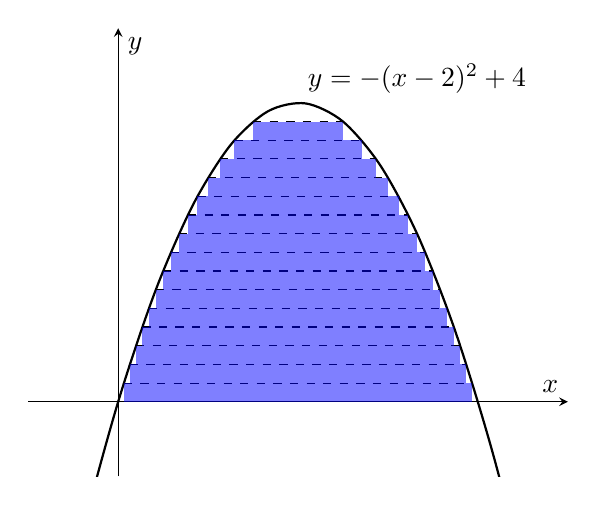
\begin{tikzpicture}[declare function={f(\x)=-(\x-2)^2+4;}]
    
                \begin{axis}[
                        axis x line=middle,
                        axis y line=middle,
                        axis line style={=>},
                        xmin=-1,xmax=5,
                        ymin=-1,ymax=5,
                        xlabel=$x$,
                        ylabel=$y$,
                        xtick=\empty,
                        ytick=\empty,
                        xticklabels=\empty,
                        yticklabels=\empty,
                    ]
                    \addplot[smooth, thick, black]{f(x)};

                    \draw[dashed] (2-1.936491673103708, 0.25) -- (2+1.936491673103708, 0.25);
                    \draw[dashed] (2-1.870828693386971, 0.5) -- (2+1.870828693386971, 0.5);
                    \draw[dashed] (2-1.802775637731995, 0.75) -- (2+1.802775637731995, 0.75);
                    \draw[dashed] (2-1.732050807568877, 1) -- (2+1.732050807568877, 1);
                    \draw[dashed] (2-1.6583123951777, 1.25) -- (2+1.6583123951777, 1.25);
                    \draw[dashed] (2-1.58113883008419, 1.5) -- (2+1.58113883008419, 1.5);
                    \draw[dashed] (2-1.5, 1.75) -- (2+1.5, 1.75);
                    \draw[dashed] (2-1.414213562373095, 2) -- (2+1.414213562373095, 2);
                    \draw[dashed] (2-1.322875655532295, 2.25) -- (2+1.322875655532295, 2.25);
                    \draw[dashed] (2-1.224744871391589, 2.5) -- (2+1.224744871391589, 2.5);
                    \draw[dashed] (2-1.118033988749895, 2.75) -- (2+1.118033988749895, 2.75);
                    \draw[dashed] (2-1, 3) -- (2+1, 3);
                    \draw[dashed] (2-0.8660254037844386, 3.25) -- (2+0.8660254037844386, 3.25);
                    \draw[dashed] (2-0.7071067811865475, 3.5) -- (2+0.7071067811865475, 3.5);
                    \draw[dashed] (2-0.5, 3.75) -- (2+0.5, 3.75);
                    \draw[dashed] (2, 4) node[above right]{$y=-(x-2)^2+4$};
                    
                    \path[fill=blue, opacity=0.5] (2-1.936491673103708, 0.25) -- (2+1.936491673103708, 0.25) -- (2+1.936491673103708, 0) -- (2-1.936491673103708, 0);
                    \path[fill=blue, opacity=0.5] (2-1.870828693386971, 0.5) -- (2+1.870828693386971, 0.5) -- (2+1.870828693386971, 0.25) -- (2-1.870828693386971, 0.25);
                    \path[fill=blue, opacity=0.5] (2-1.802775637731995, 0.75) -- (2+1.802775637731995, 0.75) -- (2+1.802775637731995, 0.5) -- (2-1.802775637731995, 0.5);
                    \path[fill=blue, opacity=0.5] (2-1.732050807568877, 1) -- (2+1.732050807568877, 1) -- (2+1.732050807568877, 0.75) -- (2-1.732050807568877, 0.75);
                    \path[fill=blue, opacity=0.5] (2-1.6583123951777, 1.25) -- (2+1.6583123951777, 1.25) -- (2+1.6583123951777, 1) -- (2-1.6583123951777, 1);
                    \path[fill=blue, opacity=0.5] (2-1.58113883008419, 1.5) -- (2+1.58113883008419, 1.5) -- (2+1.58113883008419, 1.25) -- (2-1.58113883008419, 1.25);
                    \path[fill=blue, opacity=0.5] (2-1.5, 1.75) -- (2+1.5, 1.75) -- (2+1.5, 1.5) -- (2-1.5, 1.5);
                    \path[fill=blue, opacity=0.5] (2-1.414213562373095, 2) -- (2+1.414213562373095, 2) -- (2+1.414213562373095, 1.75) -- (2-1.414213562373095, 1.75);
                    \path[fill=blue, opacity=0.5] (2-1.322875655532295, 2.25) -- (2+1.322875655532295, 2.25) -- (2+1.322875655532295, 2) -- (2-1.322875655532295, 2);
                    \path[fill=blue, opacity=0.5] (2-1.224744871391589, 2.5) -- (2+1.224744871391589, 2.5) -- (2+1.224744871391589, 2.25) -- (2-1.224744871391589, 2.25);
                    \path[fill=blue, opacity=0.5] (2-1.118033988749895, 2.75) -- (2+1.118033988749895, 2.75) -- (2+1.118033988749895, 2.5) -- (2-1.118033988749895, 2.5);
                    \path[fill=blue, opacity=0.5] (2-1, 3) -- (2+1, 3) -- (2+1, 2.75) -- (2-1, 2.75);
                    \path[fill=blue, opacity=0.5] (2-0.8660254037844386, 3.25) -- (2+0.8660254037844386, 3.25) -- (2+0.8660254037844386, 3) -- (2-0.8660254037844386, 3);
                    \path[fill=blue, opacity=0.5] (2-0.7071067811865475, 3.5) -- (2+0.7071067811865475, 3.5) -- (2+0.7071067811865475, 3.25) -- (2-0.7071067811865475, 3.25);
                    \path[fill=blue, opacity=0.5] (2-0.5, 3.75) -- (2+0.5, 3.75) -- (2+0.5, 3.5) -- (2-0.5, 3.5);
                \end{axis}
                
            \end{tikzpicture}

        \end{center}

        The volumes of the rectangles are $y\cdot m(f^{-1}(y))$.
        When is this useful?

    \end{frame}

    \begin{frame}{Measure Theory}

        For a set $X$, a \textbf{measure} is a function $\mu:X\rightarrow[0, \infty]$ such that\pause

        \begin{enumerate}
            \item A subset $E\subseteq X$ has non-negative measure $\mu(E)\geq0$,\pause
            \item The empty set has empty measure $\mu(\emptyset)=0$,\pause
            \item For a \textbf{countable} number of \textbf{disjoint} sets, we have countable sub-additivity, i.e. we can measure them individually

            \[\mu\left(\bigcup_{k=1}^\infty E_k\right)=\sum_{k=1}^\infty \mu(E_k).\]
        \end{enumerate}

        \pause

        \vspace{24pt}

        The \textbf{Lebesgue measure} is a special measure $m:\mathbb{R}\rightarrow[0, \infty]$ ALSO satisfying:\pause

        \begin{enumerate}
            \item $m([a, b])=b-a$,\pause
            \item Translation invariance $m(E)=m(E+t)$.
        \end{enumerate}
        
    \end{frame}

    \begin{frame}{Integrating (Lebesgue Style)}

        Again taking

        \[1_\mathbb{Q}=\begin{cases}
            1\quad\text{if}\;x\in\mathbb{Q}\\
            0\quad\text{else}
        \end{cases}\quad\quad\text{and}\quad\quad 1_{\mathbb{R}\setminus\mathbb{Q}}=\begin{cases}
            0\quad\text{if}\;x\in\mathbb{Q}\\
            1\quad\text{else}
        \end{cases}\]\pause
        the integral under the Lebesgue measure can easily be calculated as

        \begin{align*}
            \int_\mathbb{R} 1_\mathbb{Q}\;dm&=0\cdot m(1_\mathbb{Q}^{-1}(0))+1\cdot m(1_\mathbb{Q}^{-1}(1))\\\pause
            &=0\cdot m(\mathbb{R}\setminus\mathbb{Q})+1\cdot m(\mathbb{Q})\\\pause
            &=m(\mathbb{Q})\\\pause
            &=\sum_{a\in\mathbb{Q}} m([a, a])\\\pause
            &=\sum_{a\in\mathbb{Q}}0\\\pause
            &=0.
        \end{align*}\pause
        Similarly (with a slight lie),

        \[\int_\mathbb{R} 1_{\mathbb{R}\setminus\mathbb{Q}}\;dm=m(\mathbb{R}\setminus\mathbb{Q})=m(\mathbb{R})-m(\mathbb{Q})=\infty.\]
        
    \end{frame}

    \addtocounter{theorem}{1}

    \begin{frame}{Measure Theory in 30 Seconds}

        \definition{A function $f(x):X\rightarrow Y$ is \textbf{$\mu$-integrable} if $\int_X \abs*{f(x)}\;d\mu<\infty$.}\pause

        \addtocounter{definition}{-1}

        \theorem{\textbf{Lebesgue-Vitali (1907)} A function $f:\mathbb{R}\rightarrow\mathbb{R}$ is Riemann integrable on $[a, b]$ if and only if it is continuous almost everywhere (that is, on $[a, b]\setminus S$ where $m(S)=0$)}.\pause

        \theorem{\textbf{Monotone Convergence Theorem} Let $(f_n)_{n\in\mathbb{N}}$ be a sequence of (a.e.) increasing measurable functions, then $f_n\rightarrow f$ is measurable, and
        \[\lim_{n\rightarrow\infty}\int_X f_n\;d\mu=\int_X \lim_{n\rightarrow\infty} f_n\;d\mu=\int_X f\;d\mu.\]}\pause

        \theorem{\textbf{Fubini/Tonelli's Theorem} If $f:\mathbb{R}^n\times\mathbb{R}^m\rightarrow\mathbb{R}$ is measurable and one of the following are finite: $\int_{\mathbb{R}^{n\times m}} \abs*{f(x, y)}\;d(x, y), \int_{\mathbb{R}^m}\left(\int_{\mathbb{R}^n} \abs*{f(x, y)}\;dx\right)\;dy, \int_{\mathbb{R}^n}\left(\int_{\mathbb{R}^m} \abs*{f(x, y)}\;dy\right)\;dx$, then
        \[\int_{\mathbb{R}^{n\times m}} f(x, y)\;d(x, y)=\int_{\mathbb{R}^m}\left(\int_{\mathbb{R}^n} f(x, y)\;dx\right)\;dy=\int_{\mathbb{R}^n}\left(\int_{\mathbb{R}^m} f(x, y)\;dy\right)\;dx.\]}
        
    \end{frame}

    \begin{frame}{What These Are In Riemann Land}
    
        \[\int_{-\infty}^\infty 1_\mathbb{Q}\;dx=\int_{-\infty}^\infty \sum_{a\in\mathbb{Q}} 1_a=\sum_{a\in\mathbb{Q}}\int_{-\infty}^\infty 1_a=\sum_{a\in\mathbb{Q}} \int_a^a 1\;dx=\sum_{a\in\mathbb{Q}} (a-a)=0.\]\pause

        \[\int_{-\infty}^\infty 1_{\mathbb{R}\setminus\mathbb{Q}}\;dx=\int_{-\infty}^\infty \sum_{a\in\mathbb{R}\setminus\mathbb{Q}} 1_a=\sum_{a\in\mathbb{R}\setminus\mathbb{Q}}\int_{-\infty}^\infty 1_a=\sum_{a\in\mathbb{R}\setminus\mathbb{Q}} \int_a^a 1\;dx=\sum_{a\in\mathbb{R}\setminus\mathbb{Q}} (a-a)=0.\]
        something is wrong... \pause WE CANNOT APPLY TONELLI'S THEOREM! \pause
        But, with the Lebesgue integral, we can!

    \end{frame}

    \begin{frame}{What These Are In Riemann Land}

        \setcounter{theorem}{2}

        \theorem{\textbf{Monotone Convergence Theorem} Let $(f_n)_{n\in\mathbb{N}}$ be a sequence of (a.e.) increasing measurable functions, then $f_n\rightarrow f$ is measurable, and
        \[\lim_{n\rightarrow\infty}\int_X f_n\;d\mu=\int_X \lim_{n\rightarrow\infty} f_n\;d\mu=\int_X f\;d\mu.\]}

        This does not even exist! \pause
        Take $(f_n)_{n\in\mathbb{Q}\cap[0, 1]}$ with

        \[f_n(x)=\begin{cases}
            1\quad\text{if}\;x\leq n\\
            0\quad\text{else}
        \end{cases}\]
        each of which have Riemann integral $0$. \pause
        $f_n$ converges to $1_{\mathbb{Q}\cap[0, 1]}$, but this is not Riemann integrable, the MCT fails in Riemann integration.
        
    \end{frame}

    \begin{frame}{What These Are In Riemann Land}

        \theorem{\textbf{Fubini/Tonelli's Theorem} If $f:\mathbb{R}^n\times\mathbb{R}^m\rightarrow\mathbb{R}$ is measurable and one of the following are finite: $\int_{\mathbb{R}^{n\times m}} \abs*{f(x, y)}\;d(x, y), \int_{\mathbb{R}^m}\left(\int_{\mathbb{R}^n} \abs*{f(x, y)}\;dx\right)\;dy, \int_{\mathbb{R}^n}\left(\int_{\mathbb{R}^m} \abs*{f(x, y)}\;dy\right)\;dx$, then
        \[\int_{\mathbb{R}^{n\times m}} f(x, y)\;d(x, y)=\int_{\mathbb{R}^m}\left(\int_{\mathbb{R}^n} f(x, y)\;dx\right)\;dy=\int_{\mathbb{R}^n}\left(\int_{\mathbb{R}^m} f(x, y)\;dy\right)\;dx.\]}

        The integrals can be swapped on a rectangle $[a, b]\times[c, d]$ if $f(x, y)$ is continuous, that is

        \[\int_a^b\left(\int_c^d f(x, y)\;dx\right)\;dy=\int_c^d\left(\int_a^b f(x, y)\;dy\right)\;dx.\]\pause

        Fubini/Tonelli's theorem is a lot less restrictive!
        
    \end{frame}

    \begin{frame}{A Special Subset of $[0, 1]$}

        \begin{center}
    
            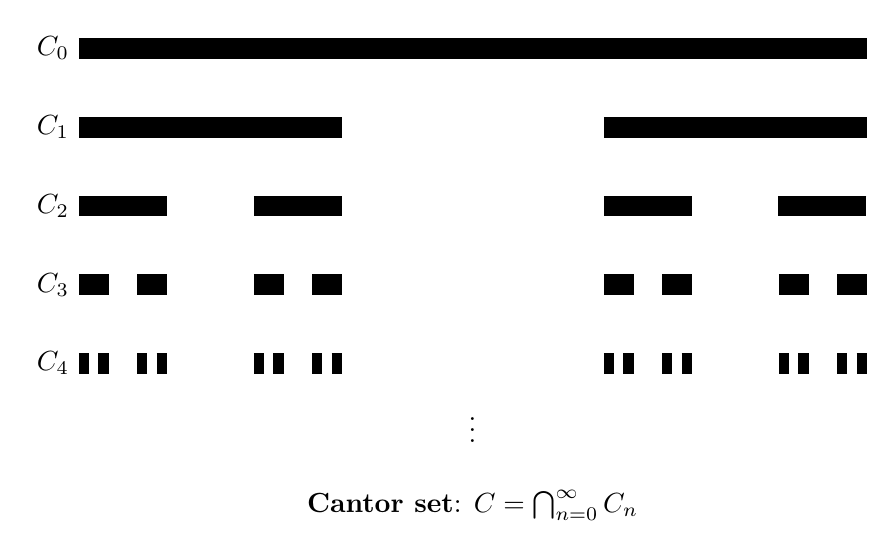
\begin{tikzpicture}

                \pause
    
                \draw[fill=black] (0, 0) -- (10, 0) -- (10, -0.25) -- (0, -0.25);

                \draw (0, -0.125) node[left]{$C_0$};

                \pause
                
                \draw[fill=black] (0, -1) -- (10/3, -1) -- (10/3, -1.25) -- (0, -1.25);
                \draw[fill=black] (20/3, -1) -- (10, -1) -- (10, -1.25) -- (20/3, -1.25);

                \draw (0, -1.125) node[left]{$C_1$};

                \pause
    
                \draw[fill=black] (0, -2) -- (10/9, -2) -- (10/9, -2.25) -- (0, -2.25);
                \draw[fill=black] (20/9, -2) -- (10/3, -2) -- (10/3, -2.25) -- (20/9, -2.25);
                \draw[fill=black] (20/3, -2) -- (20/3+10/9, -2) -- (20/3+10/9, -2.25) -- (20/3, -2.25);
                \draw[fill=black] (10, -2) -- (20/3+20/9, -2) -- (20/3+20/9, -2.25) -- (10, -2.25);

                \draw (0, -2.125) node[left]{$C_2$};

                \pause
    
                \draw[fill=black] (0, -3) -- (10/27, -3) -- (10/27, -3.25) -- (0, -3.25);
                \draw[fill=black] (20/27, -3) -- (10/9, -3) -- (10/9, -3.25) -- (20/27, -3.25);
                \draw[fill=black] (0+20/9, -3) -- (10/27+20/9, -3) -- (10/27+20/9, -3.25) -- (0+20/9, -3.25);
                \draw[fill=black] (20/27+20/9, -3) -- (10/9+20/9, -3) -- (10/9+20/9, -3.25) -- (20/27+20/9, -3.25);
                \draw[fill=black] (0+20/3, -3) -- (10/27+20/3, -3) -- (10/27+20/3, -3.25) -- (0+20/3, -3.25);
                \draw[fill=black] (20/27+20/3, -3) -- (10/9+20/3, -3) -- (10/9+20/3, -3.25) -- (20/27+20/3, -3.25);
                \draw[fill=black] (0+20/9+20/3, -3) -- (10/27+20/9+20/3, -3) -- (10/27+20/9+20/3, -3.25) -- (0+20/9+20/3, -3.25);
                \draw[fill=black] (20/27+20/9+20/3, -3) -- (10/9+20/9+20/3, -3) -- (10/9+20/9+20/3, -3.25) -- (20/27+20/9+20/3, -3.25);

                \draw (0, -3.125) node[left]{$C_3$};

                \pause
    
                \draw[fill=black] (0, -4) -- (10/81, -4) -- (10/81, -4.25) -- (0, -4.25);
                \draw[fill=black] (20/81, -4) -- (10/81+20/81, -4) -- (10/81+20/81, -4.25) -- (20/81, -4.25);
                \draw[fill=black] (0+20/27, -4) -- (10/81+20/27, -4) -- (10/81+20/27, -4.25) -- (0+20/27, -4.25);
                \draw[fill=black] (20/81+20/27, -4) -- (10/81+20/81+20/27, -4) -- (10/81+20/81+20/27, -4.25) -- (20/81+20/27, -4.25);
                \draw[fill=black] (0+20/9, -4) -- (10/81+20/9, -4) -- (10/81+20/9, -4.25) -- (0+20/9, -4.25);
                \draw[fill=black] (20/81+20/9, -4) -- (10/81+20/81+20/9, -4) -- (10/81+20/81+20/9, -4.25) -- (20/81+20/9, -4.25);
                \draw[fill=black] (0+20/27+20/9, -4) -- (10/81+20/27+20/9, -4) -- (10/81+20/27+20/9, -4.25) -- (0+20/27+20/9, -4.25);
                \draw[fill=black] (20/81+20/27+20/9, -4) -- (10/81+20/81+20/27+20/9, -4) -- (10/81+20/81+20/27+20/9, -4.25) -- (20/81+20/27+20/9, -4.25);
                \draw[fill=black] (0+20/3, -4) -- (10/81+20/3, -4) -- (10/81+20/3, -4.25) -- (0+20/3, -4.25);
                \draw[fill=black] (20/81+20/3, -4) -- (10/81+20/81+20/3, -4) -- (10/81+20/81+20/3, -4.25) -- (20/81+20/3, -4.25);
                \draw[fill=black] (0+20/27+20/3, -4) -- (10/81+20/27+20/3, -4) -- (10/81+20/27+20/3, -4.25) -- (0+20/27+20/3, -4.25);
                \draw[fill=black] (20/81+20/27+20/3, -4) -- (10/81+20/81+20/27+20/3, -4) -- (10/81+20/81+20/27+20/3, -4.25) -- (20/81+20/27+20/3, -4.25);
                \draw[fill=black] (0+20/9+20/3, -4) -- (10/81+20/9+20/3, -4) -- (10/81+20/9+20/3, -4.25) -- (0+20/9+20/3, -4.25);
                \draw[fill=black] (20/81+20/9+20/3, -4) -- (10/81+20/81+20/9+20/3, -4) -- (10/81+20/81+20/9+20/3, -4.25) -- (20/81+20/9+20/3, -4.25);
                \draw[fill=black] (0+20/27+20/9+20/3, -4) -- (10/81+20/27+20/9+20/3, -4) -- (10/81+20/27+20/9+20/3, -4.25) -- (0+20/27+20/9+20/3, -4.25);
                \draw[fill=black] (20/81+20/27+20/9+20/3, -4) -- (10/81+20/81+20/27+20/9+20/3, -4) -- (10/81+20/81+20/27+20/9+20/3, -4.25) -- (20/81+20/27+20/9+20/3, -4.25);

                \draw (0, -4.125) node[left]{$C_4$};

                \pause

                \draw (5, -5.25) node[above]{$\vdots$};

                \draw (5, -6.25) node[above]{\textbf{Cantor set}: $C=\bigcap_{n=0}^\infty C_n$};
                
            \end{tikzpicture}
    
        \end{center}

        \textcolor{white}{\textbf{Claim:} The Cantor set is uncountable.}
        
    \end{frame}
        
    \begin{frame}{A Special Subset of $[0, 1]$}

        \begin{center}
    
            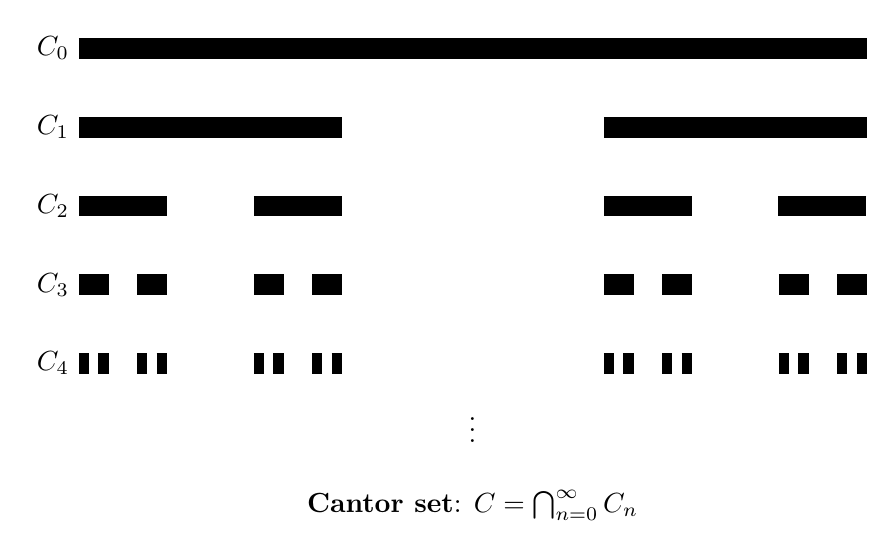
\begin{tikzpicture}

                \pause
    
                \draw[fill=black] (0, 0) -- (10, 0) -- (10, -0.25) -- (0, -0.25);

                \draw (0, -0.125) node[left]{$C_0$};

                \pause
                
                \draw[fill=black] (0, -1) -- (10/3, -1) -- (10/3, -1.25) -- (0, -1.25);
                \draw[fill=black] (20/3, -1) -- (10, -1) -- (10, -1.25) -- (20/3, -1.25);

                \draw (0, -1.125) node[left]{$C_1$};

                \pause
    
                \draw[fill=black] (0, -2) -- (10/9, -2) -- (10/9, -2.25) -- (0, -2.25);
                \draw[fill=black] (20/9, -2) -- (10/3, -2) -- (10/3, -2.25) -- (20/9, -2.25);
                \draw[fill=black] (20/3, -2) -- (20/3+10/9, -2) -- (20/3+10/9, -2.25) -- (20/3, -2.25);
                \draw[fill=black] (10, -2) -- (20/3+20/9, -2) -- (20/3+20/9, -2.25) -- (10, -2.25);

                \draw (0, -2.125) node[left]{$C_2$};

                \pause
    
                \draw[fill=black] (0, -3) -- (10/27, -3) -- (10/27, -3.25) -- (0, -3.25);
                \draw[fill=black] (20/27, -3) -- (10/9, -3) -- (10/9, -3.25) -- (20/27, -3.25);
                \draw[fill=black] (0+20/9, -3) -- (10/27+20/9, -3) -- (10/27+20/9, -3.25) -- (0+20/9, -3.25);
                \draw[fill=black] (20/27+20/9, -3) -- (10/9+20/9, -3) -- (10/9+20/9, -3.25) -- (20/27+20/9, -3.25);
                \draw[fill=black] (0+20/3, -3) -- (10/27+20/3, -3) -- (10/27+20/3, -3.25) -- (0+20/3, -3.25);
                \draw[fill=black] (20/27+20/3, -3) -- (10/9+20/3, -3) -- (10/9+20/3, -3.25) -- (20/27+20/3, -3.25);
                \draw[fill=black] (0+20/9+20/3, -3) -- (10/27+20/9+20/3, -3) -- (10/27+20/9+20/3, -3.25) -- (0+20/9+20/3, -3.25);
                \draw[fill=black] (20/27+20/9+20/3, -3) -- (10/9+20/9+20/3, -3) -- (10/9+20/9+20/3, -3.25) -- (20/27+20/9+20/3, -3.25);

                \draw (0, -3.125) node[left]{$C_3$};

                \pause
    
                \draw[fill=black] (0, -4) -- (10/81, -4) -- (10/81, -4.25) -- (0, -4.25);
                \draw[fill=black] (20/81, -4) -- (10/81+20/81, -4) -- (10/81+20/81, -4.25) -- (20/81, -4.25);
                \draw[fill=black] (0+20/27, -4) -- (10/81+20/27, -4) -- (10/81+20/27, -4.25) -- (0+20/27, -4.25);
                \draw[fill=black] (20/81+20/27, -4) -- (10/81+20/81+20/27, -4) -- (10/81+20/81+20/27, -4.25) -- (20/81+20/27, -4.25);
                \draw[fill=black] (0+20/9, -4) -- (10/81+20/9, -4) -- (10/81+20/9, -4.25) -- (0+20/9, -4.25);
                \draw[fill=black] (20/81+20/9, -4) -- (10/81+20/81+20/9, -4) -- (10/81+20/81+20/9, -4.25) -- (20/81+20/9, -4.25);
                \draw[fill=black] (0+20/27+20/9, -4) -- (10/81+20/27+20/9, -4) -- (10/81+20/27+20/9, -4.25) -- (0+20/27+20/9, -4.25);
                \draw[fill=black] (20/81+20/27+20/9, -4) -- (10/81+20/81+20/27+20/9, -4) -- (10/81+20/81+20/27+20/9, -4.25) -- (20/81+20/27+20/9, -4.25);
                \draw[fill=black] (0+20/3, -4) -- (10/81+20/3, -4) -- (10/81+20/3, -4.25) -- (0+20/3, -4.25);
                \draw[fill=black] (20/81+20/3, -4) -- (10/81+20/81+20/3, -4) -- (10/81+20/81+20/3, -4.25) -- (20/81+20/3, -4.25);
                \draw[fill=black] (0+20/27+20/3, -4) -- (10/81+20/27+20/3, -4) -- (10/81+20/27+20/3, -4.25) -- (0+20/27+20/3, -4.25);
                \draw[fill=black] (20/81+20/27+20/3, -4) -- (10/81+20/81+20/27+20/3, -4) -- (10/81+20/81+20/27+20/3, -4.25) -- (20/81+20/27+20/3, -4.25);
                \draw[fill=black] (0+20/9+20/3, -4) -- (10/81+20/9+20/3, -4) -- (10/81+20/9+20/3, -4.25) -- (0+20/9+20/3, -4.25);
                \draw[fill=black] (20/81+20/9+20/3, -4) -- (10/81+20/81+20/9+20/3, -4) -- (10/81+20/81+20/9+20/3, -4.25) -- (20/81+20/9+20/3, -4.25);
                \draw[fill=black] (0+20/27+20/9+20/3, -4) -- (10/81+20/27+20/9+20/3, -4) -- (10/81+20/27+20/9+20/3, -4.25) -- (0+20/27+20/9+20/3, -4.25);
                \draw[fill=black] (20/81+20/27+20/9+20/3, -4) -- (10/81+20/81+20/27+20/9+20/3, -4) -- (10/81+20/81+20/27+20/9+20/3, -4.25) -- (20/81+20/27+20/9+20/3, -4.25);

                \draw (0, -4.125) node[left]{$C_4$};

                \pause

                \draw (5, -5.25) node[above]{$\vdots$};

                \draw (5, -6.25) node[above]{\textbf{Cantor set}: $C=\bigcap_{n=0}^\infty C_n$};
                
            \end{tikzpicture}
    
        \end{center}

        \textcolor{white}{\textbf{Claim:} The Cantor set is uncountable.}
        
    \end{frame}

    \begin{frame}{Cantor Set}

        Consider constructing some sequences by adding a decimal of $0, 1$ or $2$ if it is the first, second or third third.
        Then with our construction:

        \begin{center}
    
            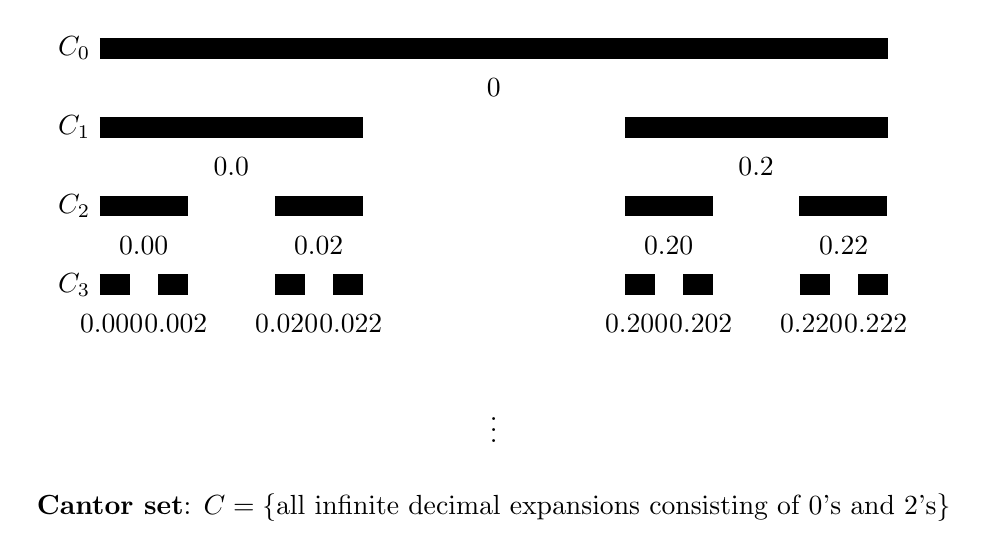
\begin{tikzpicture}

                \pause
    
                \draw[fill=black] (0, 0) -- (10, 0) -- (10, -0.25) -- (0, -0.25);

                \draw (0, -0.125) node[left]{$C_0$};

                \draw (5, -0.625) node{$0$};

                \pause
                
                \draw[fill=black] (0, -1) -- (10/3, -1) -- (10/3, -1.25) -- (0, -1.25);
                \draw[fill=black] (20/3, -1) -- (10, -1) -- (10, -1.25) -- (20/3, -1.25);

                \draw (0, -1.125) node[left]{$C_1$};

                \draw (5/3, -1.625) node{$0.0$};
                \draw (25/3, -1.625) node{$0.2$};

                \pause
    
                \draw[fill=black] (0, -2) -- (10/9, -2) -- (10/9, -2.25) -- (0, -2.25);
                \draw[fill=black] (20/9, -2) -- (10/3, -2) -- (10/3, -2.25) -- (20/9, -2.25);
                \draw[fill=black] (20/3, -2) -- (20/3+10/9, -2) -- (20/3+10/9, -2.25) -- (20/3, -2.25);
                \draw[fill=black] (10, -2) -- (20/3+20/9, -2) -- (20/3+20/9, -2.25) -- (10, -2.25);

                \draw (0, -2.125) node[left]{$C_2$};

                \draw (5/9, -2.625) node{$0.00$};
                \draw (25/9, -2.625) node{$0.02$};
                \draw (65/9, -2.625) node{$0.20$};
                \draw (85/9, -2.625) node{$0.22$};

                \pause
    
                \draw[fill=black] (0, -3) -- (10/27, -3) -- (10/27, -3.25) -- (0, -3.25);
                \draw[fill=black] (20/27, -3) -- (10/9, -3) -- (10/9, -3.25) -- (20/27, -3.25);
                \draw[fill=black] (0+20/9, -3) -- (10/27+20/9, -3) -- (10/27+20/9, -3.25) -- (0+20/9, -3.25);
                \draw[fill=black] (20/27+20/9, -3) -- (10/9+20/9, -3) -- (10/9+20/9, -3.25) -- (20/27+20/9, -3.25);
                \draw[fill=black] (0+20/3, -3) -- (10/27+20/3, -3) -- (10/27+20/3, -3.25) -- (0+20/3, -3.25);
                \draw[fill=black] (20/27+20/3, -3) -- (10/9+20/3, -3) -- (10/9+20/3, -3.25) -- (20/27+20/3, -3.25);
                \draw[fill=black] (0+20/9+20/3, -3) -- (10/27+20/9+20/3, -3) -- (10/27+20/9+20/3, -3.25) -- (0+20/9+20/3, -3.25);
                \draw[fill=black] (20/27+20/9+20/3, -3) -- (10/9+20/9+20/3, -3) -- (10/9+20/9+20/3, -3.25) -- (20/27+20/9+20/3, -3.25);

                \draw (0, -3.125) node[left]{$C_3$};

                \draw (5/27-1/27, -3.625) node{$0.000$};
                \draw (25/27+1/27, -3.625) node{$0.002$};
                \draw (65/27-1/27, -3.625) node{$0.020$};
                \draw (85/27+1/27, -3.625) node{$0.022$};
                \draw (185/27-1/27, -3.625) node{$0.200$};
                \draw (205/27+1/27, -3.625) node{$0.202$};
                \draw (245/27-1/27, -3.625) node{$0.220$};
                \draw (265/27+1/27, -3.625) node{$0.222$};

                \pause

                \draw (5, -5.25) node[above]{$\vdots$};

                \draw (5, -6.25) node[above]{\textbf{Cantor set}: $C=\{\text{all infinite decimal expansions consisting of $0$'s and $2$'s}\}$};
                
            \end{tikzpicture}
    
        \end{center}
        
    \end{frame}

    \begin{frame}{Cantor Function}

        These are called \textbf{ternary expansions}, i.e. writing the decimal base $3$.
        So the cantor set is precisely the ternary expansions in $[0, 1]$ which do not contain $1$.

        \pause

        \vspace{24pt}

        The \textbf{cantor function} $c$ maps such ternary expansions to \textbf{binary expansions} by replacing $2$ with $1$ (and connecting the gaps).
        So

        \begin{align*}
            C&=\{\text{all infinite decimal expansions consisting of $0$'s and $2$'s}\}\\\pause
            \Rightarrow c(C)&=\{\text{all infinite decimal expansions consisting of $0$'s and $1$'s}\}\\\pause
            &=\{\text{all binary decimal expansions}\}\\\pause
            &=[0, 1]
        \end{align*}
        and thus $C$ must be uncountable. \pause
        Now

        \[m(C_n)=\left(\frac{2}{3}\right)^n\pause\Rightarrow m(C)=\lim_{n\rightarrow\infty} \left(\frac{2}{3}\right)^n=0.\]
        
    \end{frame}

    \begin{frame}{Cantor Function is Weird}

        \begin{figure}

            \begin{center}

                \includegraphics[width=0.6\linewidth]{CantorEscalier-2.png}

            \end{center}
            
        \end{figure}

        $c$ is continuous, but not absolutely continuous.
        It is not differentiable on $\mathbb{R}$-INFINITELY many points, but has zero derivative almost everywhere.
        
    \end{frame}

\begin{frame}{Can All Sets be (Lebesgue) Measured?}

        Start with the unit interval $[0, 1]$ and partition it into equivalence classes where:

        \[a\sim b\Leftrightarrow a-b\in\mathbb{Q}\]
        so for example, $\frac{\pi}{4}\sim\frac{\pi}{4}+\frac{1}{123}\sim\frac{\pi}{4}+\frac{1}{2}\sim\dots$. \pause
        These equivalence classes $[a]$ are represented by one singular irrational number $a$ (or $0$) and all sums of rational numbers (in $[0, 1]$), i.e. by the set

        \[a+\mathbb{Q}=\{a+q\;|\;q\in\mathbb{Q}\},\]
        intersected with the unit interval.

        \pause

        \vspace{24pt}
        
        We have $\mathbb{R}$-INFINITELY many of these sets (one for each irrational), and each of them contains $\mathbb{Q}$-infinitely many numbers.

        \pause

        \vspace{24pt}
        
        Moreover they are all disjoint: if there are $[a], [a']$ with some $a+q=a'+q'$ then $a-a'=q'-q\in\mathbb{Q}$ and so we must have $[a]=[a']$.
        
    \end{frame}

    \begin{frame}{Set Theory}

        The \textbf{Zermelo-Fraenkel axioms} of set theory are a set of $8$ rules we accept to be true.

        \pause

        \vspace{24pt}

        \textbf{The Axiom of Choice}: Given a (possibly infinite) collection of non-empty sets, we can choose one element from each of them.

        \pause

        \vspace{24pt}

        Whilst this seems obvious, it is impossible to prove this from the $8$ axioms of ZF set theory, so with this 9th axiom, we have ZFC set theory.
        In measure theory we ACCEPT the axiom of choice.

        \pause

        \vspace{24pt}

        Using the axiom of choice, and our $\mathbb{R}$-INFINITELY many equivalence classes $[a]$, we can choose one from each to form a new set $V$ called the \textbf{Vitali set}.
        
    \end{frame}

    \begin{frame}{Measure of the Vitali Set}

        We now want to consider the set $V_q:=V+q$ for all $q\in\mathbb{Q}\cap[-1, 1]$ which translates all elements in $V$ by $q$.

        \begin{center}

            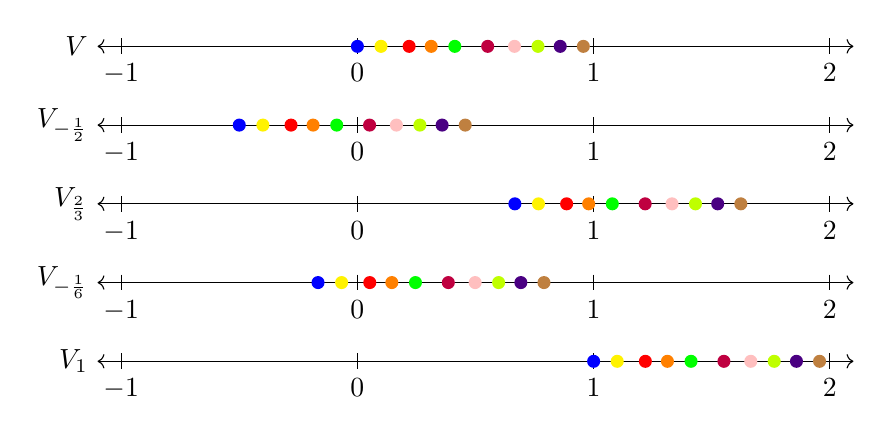
\begin{tikzpicture}
    
                \draw[<->, fill=black] (-3.3, 0) node[left]{$V$} -- (6.3, 0);
                \draw (0, 0.1) -- (0, -0.1) node[below]{$0$};
                \draw (-3, 0.1) -- (-3, -0.1) node[below]{$-1$};
                \draw (3, 0.1) -- (3, -0.1) node[below]{$1$};
                \draw (6, 0.1) -- (6, -0.1) node[below]{$2$};

                \draw (0, 0) node[fill=blue, shape=circle, scale=0.5]{};
                \draw (0.2998, 0) node[fill=yellow, shape=circle, scale=0.5]{};
                \draw (0.6571, 0) node[fill=red, shape=circle, scale=0.5]{};
                \draw (0.93729, 0) node[fill=orange, shape=circle, scale=0.5]{};
                \draw (1.2373, 0) node[fill=green, shape=circle, scale=0.5]{};
                \draw (1.65467, 0) node[fill=purple, shape=circle, scale=0.5]{};
                \draw (1.9957, 0) node[fill=pink, shape=circle, scale=0.5]{};
                \draw (2.2937, 0) node[fill=lime, shape=circle, scale=0.5]{};
                \draw (2.5759, 0) node[fill=indigo, shape=circle, scale=0.5]{};
                \draw (2.8695, 0) node[fill=brown, shape=circle, scale=0.5]{};

                \pause

                \draw[<->, fill=black] (-3.3, -1) node[left]{$V_{-\frac{1}{2}}$} -- (6.3, -1);
                \draw (0, 0.1-1) -- (0, -0.1-1) node[below]{$0$};
                \draw (-3, 0.1-1) -- (-3, -0.1-1) node[below]{$-1$};
                \draw (3, 0.1-1) -- (3, -0.1-1) node[below]{$1$};
                \draw (6, 0.1-1) -- (6, -0.1-1) node[below]{$2$};

                \draw (0-1.5, -1) node[fill=blue, shape=circle, scale=0.5]{};
                \draw (0.2998-1.5, -1) node[fill=yellow, shape=circle, scale=0.5]{};
                \draw (0.6571-1.5, -1) node[fill=red, shape=circle, scale=0.5]{};
                \draw (0.93729-1.5, -1) node[fill=orange, shape=circle, scale=0.5]{};
                \draw (1.2373-1.5, -1) node[fill=green, shape=circle, scale=0.5]{};
                \draw (1.65467-1.5, -1) node[fill=purple, shape=circle, scale=0.5]{};
                \draw (1.9957-1.5, -1) node[fill=pink, shape=circle, scale=0.5]{};
                \draw (2.2937-1.5, -1) node[fill=lime, shape=circle, scale=0.5]{};
                \draw (2.5759-1.5, -1) node[fill=indigo, shape=circle, scale=0.5]{};
                \draw (2.8695-1.5, -1) node[fill=brown, shape=circle, scale=0.5]{};

                \pause

                \draw[<->, fill=black] (-3.3, -2) node[left]{$V_{\frac{2}{3}}$} -- (6.3, -2);
                \draw (0, 0.1-2) -- (0, -0.1-2) node[below]{$0$};
                \draw (-3, 0.1-2) -- (-3, -0.1-2) node[below]{$-1$};
                \draw (3, 0.1-2) -- (3, -0.1-2) node[below]{$1$};
                \draw (6, 0.1-2) -- (6, -0.1-2) node[below]{$2$};

                \draw (0+2, -2) node[fill=blue, shape=circle, scale=0.5]{};
                \draw (0.2998+2, -2) node[fill=yellow, shape=circle, scale=0.5]{};
                \draw (0.6571+2, -2) node[fill=red, shape=circle, scale=0.5]{};
                \draw (0.93729+2, -2) node[fill=orange, shape=circle, scale=0.5]{};
                \draw (1.2373+2, -2) node[fill=green, shape=circle, scale=0.5]{};
                \draw (1.65467+2, -2) node[fill=purple, shape=circle, scale=0.5]{};
                \draw (1.9957+2, -2) node[fill=pink, shape=circle, scale=0.5]{};
                \draw (2.2937+2, -2) node[fill=lime, shape=circle, scale=0.5]{};
                \draw (2.5759+2, -2) node[fill=indigo, shape=circle, scale=0.5]{};
                \draw (2.8695+2, -2) node[fill=brown, shape=circle, scale=0.5]{};

                \pause

                \draw[<->, fill=black] (-3.3, -3) node[left]{$V_{-\frac{1}{6}}$} -- (6.3, -3);
                \draw (0, 0.1-3) -- (0, -0.1-3) node[below]{$0$};
                \draw (-3, 0.1-3) -- (-3, -0.1-3) node[below]{$-1$};
                \draw (3, 0.1-3) -- (3, -0.1-3) node[below]{$1$};
                \draw (6, 0.1-3) -- (6, -0.1-3) node[below]{$2$};

                \draw (0-0.5, -3) node[fill=blue, shape=circle, scale=0.5]{};
                \draw (0.2998-0.5, -3) node[fill=yellow, shape=circle, scale=0.5]{};
                \draw (0.6571-0.5, -3) node[fill=red, shape=circle, scale=0.5]{};
                \draw (0.93729-0.5, -3) node[fill=orange, shape=circle, scale=0.5]{};
                \draw (1.2373-0.5, -3) node[fill=green, shape=circle, scale=0.5]{};
                \draw (1.65467-0.5, -3) node[fill=purple, shape=circle, scale=0.5]{};
                \draw (1.9957-0.5, -3) node[fill=pink, shape=circle, scale=0.5]{};
                \draw (2.2937-0.5, -3) node[fill=lime, shape=circle, scale=0.5]{};
                \draw (2.5759-0.5, -3) node[fill=indigo, shape=circle, scale=0.5]{};
                \draw (2.8695-0.5, -3) node[fill=brown, shape=circle, scale=0.5]{};

                \pause

                \draw[<->, fill=black] (-3.3, -4) node[left]{$V_1$} -- (6.3, -4);
                \draw (0, 0.1-4) -- (0, -0.1-4) node[below]{$0$};
                \draw (-3, 0.1-4) -- (-3, -0.1-4) node[below]{$-1$};
                \draw (3, 0.1-4) -- (3, -0.1-4) node[below]{$1$};
                \draw (6, 0.1-4) -- (6, -0.1-4) node[below]{$2$};

                \draw (0+3, -4) node[fill=blue, shape=circle, scale=0.5]{};
                \draw (0.2998+3, -4) node[fill=yellow, shape=circle, scale=0.5]{};
                \draw (0.6571+3, -4) node[fill=red, shape=circle, scale=0.5]{};
                \draw (0.93729+3, -4) node[fill=orange, shape=circle, scale=0.5]{};
                \draw (1.2373+3, -4) node[fill=green, shape=circle, scale=0.5]{};
                \draw (1.65467+3, -4) node[fill=purple, shape=circle, scale=0.5]{};
                \draw (1.9957+3, -4) node[fill=pink, shape=circle, scale=0.5]{};
                \draw (2.2937+3, -4) node[fill=lime, shape=circle, scale=0.5]{};
                \draw (2.5759+3, -4) node[fill=indigo, shape=circle, scale=0.5]{};
                \draw (2.8695+3, -4) node[fill=brown, shape=circle, scale=0.5]{};
                
            \end{tikzpicture}

        \end{center}

        \textcolor{white}{There are $\mathbb{Q}$-infinitely many $V_q$'s, and they are disjoint for the same reason as the $[a]$'s.}
        
    \end{frame}

\begin{frame}{Measure of the Vitali Set}

        We now want to consider the set $V_q:=V+q$ for all $q\in\mathbb{Q}\cap[-1, 1]$ which translates all elements in $V$ by $q$.

        \begin{center}

            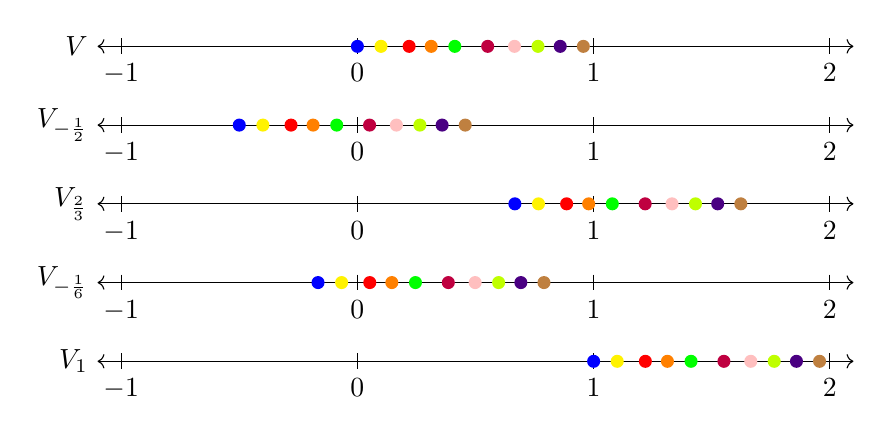
\begin{tikzpicture}
    
                \draw[<->, fill=black] (-3.3, 0) node[left]{$V$} -- (6.3, 0);
                \draw (0, 0.1) -- (0, -0.1) node[below]{$0$};
                \draw (-3, 0.1) -- (-3, -0.1) node[below]{$-1$};
                \draw (3, 0.1) -- (3, -0.1) node[below]{$1$};
                \draw (6, 0.1) -- (6, -0.1) node[below]{$2$};

                \draw (0, 0) node[fill=blue, shape=circle, scale=0.5]{};
                \draw (0.2998, 0) node[fill=yellow, shape=circle, scale=0.5]{};
                \draw (0.6571, 0) node[fill=red, shape=circle, scale=0.5]{};
                \draw (0.93729, 0) node[fill=orange, shape=circle, scale=0.5]{};
                \draw (1.2373, 0) node[fill=green, shape=circle, scale=0.5]{};
                \draw (1.65467, 0) node[fill=purple, shape=circle, scale=0.5]{};
                \draw (1.9957, 0) node[fill=pink, shape=circle, scale=0.5]{};
                \draw (2.2937, 0) node[fill=lime, shape=circle, scale=0.5]{};
                \draw (2.5759, 0) node[fill=indigo, shape=circle, scale=0.5]{};
                \draw (2.8695, 0) node[fill=brown, shape=circle, scale=0.5]{};

                \draw[<->, fill=black] (-3.3, -1) node[left]{$V_{-\frac{1}{2}}$} -- (6.3, -1);
                \draw (0, 0.1-1) -- (0, -0.1-1) node[below]{$0$};
                \draw (-3, 0.1-1) -- (-3, -0.1-1) node[below]{$-1$};
                \draw (3, 0.1-1) -- (3, -0.1-1) node[below]{$1$};
                \draw (6, 0.1-1) -- (6, -0.1-1) node[below]{$2$};

                \draw (0-1.5, -1) node[fill=blue, shape=circle, scale=0.5]{};
                \draw (0.2998-1.5, -1) node[fill=yellow, shape=circle, scale=0.5]{};
                \draw (0.6571-1.5, -1) node[fill=red, shape=circle, scale=0.5]{};
                \draw (0.93729-1.5, -1) node[fill=orange, shape=circle, scale=0.5]{};
                \draw (1.2373-1.5, -1) node[fill=green, shape=circle, scale=0.5]{};
                \draw (1.65467-1.5, -1) node[fill=purple, shape=circle, scale=0.5]{};
                \draw (1.9957-1.5, -1) node[fill=pink, shape=circle, scale=0.5]{};
                \draw (2.2937-1.5, -1) node[fill=lime, shape=circle, scale=0.5]{};
                \draw (2.5759-1.5, -1) node[fill=indigo, shape=circle, scale=0.5]{};
                \draw (2.8695-1.5, -1) node[fill=brown, shape=circle, scale=0.5]{};

                \draw[<->, fill=black] (-3.3, -2) node[left]{$V_{\frac{2}{3}}$} -- (6.3, -2);
                \draw (0, 0.1-2) -- (0, -0.1-2) node[below]{$0$};
                \draw (-3, 0.1-2) -- (-3, -0.1-2) node[below]{$-1$};
                \draw (3, 0.1-2) -- (3, -0.1-2) node[below]{$1$};
                \draw (6, 0.1-2) -- (6, -0.1-2) node[below]{$2$};

                \draw (0+2, -2) node[fill=blue, shape=circle, scale=0.5]{};
                \draw (0.2998+2, -2) node[fill=yellow, shape=circle, scale=0.5]{};
                \draw (0.6571+2, -2) node[fill=red, shape=circle, scale=0.5]{};
                \draw (0.93729+2, -2) node[fill=orange, shape=circle, scale=0.5]{};
                \draw (1.2373+2, -2) node[fill=green, shape=circle, scale=0.5]{};
                \draw (1.65467+2, -2) node[fill=purple, shape=circle, scale=0.5]{};
                \draw (1.9957+2, -2) node[fill=pink, shape=circle, scale=0.5]{};
                \draw (2.2937+2, -2) node[fill=lime, shape=circle, scale=0.5]{};
                \draw (2.5759+2, -2) node[fill=indigo, shape=circle, scale=0.5]{};
                \draw (2.8695+2, -2) node[fill=brown, shape=circle, scale=0.5]{};

                \draw[<->, fill=black] (-3.3, -3) node[left]{$V_{-\frac{1}{6}}$} -- (6.3, -3);
                \draw (0, 0.1-3) -- (0, -0.1-3) node[below]{$0$};
                \draw (-3, 0.1-3) -- (-3, -0.1-3) node[below]{$-1$};
                \draw (3, 0.1-3) -- (3, -0.1-3) node[below]{$1$};
                \draw (6, 0.1-3) -- (6, -0.1-3) node[below]{$2$};

                \draw (0-0.5, -3) node[fill=blue, shape=circle, scale=0.5]{};
                \draw (0.2998-0.5, -3) node[fill=yellow, shape=circle, scale=0.5]{};
                \draw (0.6571-0.5, -3) node[fill=red, shape=circle, scale=0.5]{};
                \draw (0.93729-0.5, -3) node[fill=orange, shape=circle, scale=0.5]{};
                \draw (1.2373-0.5, -3) node[fill=green, shape=circle, scale=0.5]{};
                \draw (1.65467-0.5, -3) node[fill=purple, shape=circle, scale=0.5]{};
                \draw (1.9957-0.5, -3) node[fill=pink, shape=circle, scale=0.5]{};
                \draw (2.2937-0.5, -3) node[fill=lime, shape=circle, scale=0.5]{};
                \draw (2.5759-0.5, -3) node[fill=indigo, shape=circle, scale=0.5]{};
                \draw (2.8695-0.5, -3) node[fill=brown, shape=circle, scale=0.5]{};

                \draw[<->, fill=black] (-3.3, -4) node[left]{$V_1$} -- (6.3, -4);
                \draw (0, 0.1-4) -- (0, -0.1-4) node[below]{$0$};
                \draw (-3, 0.1-4) -- (-3, -0.1-4) node[below]{$-1$};
                \draw (3, 0.1-4) -- (3, -0.1-4) node[below]{$1$};
                \draw (6, 0.1-4) -- (6, -0.1-4) node[below]{$2$};

                \draw (0+3, -4) node[fill=blue, shape=circle, scale=0.5]{};
                \draw (0.2998+3, -4) node[fill=yellow, shape=circle, scale=0.5]{};
                \draw (0.6571+3, -4) node[fill=red, shape=circle, scale=0.5]{};
                \draw (0.93729+3, -4) node[fill=orange, shape=circle, scale=0.5]{};
                \draw (1.2373+3, -4) node[fill=green, shape=circle, scale=0.5]{};
                \draw (1.65467+3, -4) node[fill=purple, shape=circle, scale=0.5]{};
                \draw (1.9957+3, -4) node[fill=pink, shape=circle, scale=0.5]{};
                \draw (2.2937+3, -4) node[fill=lime, shape=circle, scale=0.5]{};
                \draw (2.5759+3, -4) node[fill=indigo, shape=circle, scale=0.5]{};
                \draw (2.8695+3, -4) node[fill=brown, shape=circle, scale=0.5]{};
                
            \end{tikzpicture}

        \end{center}

        There are $\mathbb{Q}$-infinitely many $V_q$'s, and they are disjoint for the same reason as the $[a]$'s.
        
    \end{frame}

   \begin{frame}{Measure of the Vitali Set}

        \textbf{Claim}: $[0, 1]\subseteq\bigcup_{q\in\mathbb{Q}\cap[-1, 1]} V_q$.

        \pause

        \vspace{24pt}

        Why?
        Take $a\in[0, 1]$, then $a\in[a_V]$ where $a_V$ is the representative chosen by the axiom of choice to be in the Vitali set. \pause
        So

        \[a=a_V+q\]
        for some $q\in[-1, 1]$ and thus $a\in V_q$.
        \hspace*{\fill}\qedsymbol

        \pause

        \vspace{24pt}

        Also, as $V_q\in[-1, 2]$ for all $q\in\mathbb{Q}\cap[-1, 1]$, so is their union, so in fact

        \[[0, 1]\subseteq\bigcup_{q\in\mathbb{Q}\cap[-1, 1]} V_q\subseteq[-1, 2].\]\pause
        Finally, remember that $m(V_q)=m(V)$ by translation invariance.
        
    \end{frame}

    \begin{frame}{Measure of the Vitali Set}

        \[[0, 1]\subseteq\bigcup_{q\in\mathbb{Q}\cap[-1, 1]} V_q\subseteq[-1, 2]\]\pause
        This inequality tells us that

        \[m([0, 1])\leq m\left(\bigcup_{q\in\mathbb{Q}\cap[-1, 1]} V_q\right)\leq m([-1, 2]).\]\pause
        By countable subadditivity and translation invariance

        \[1\leq \sum_{q\in\mathbb{Q}\cap[-1, 1]} m(V)\leq 3.\]\pause

        So what is the measure of $V$?\pause

        \begin{itemize}
            \item If $m(V)=0\Rightarrow\sum_{q\in\mathbb{Q}\cap[-1, 1]} m(V)=0$, but it must be at least $1$. \pause
            \item If $m(V)=\varepsilon>0\Rightarrow\sum_{q\in\mathbb{Q}\cap[-1, 1]} m(V)=\infty$, but it must be at most $3$.
        \end{itemize}

        \pause

        \vspace{24pt}

        Logical conclusion?
        The Vitali set $V$ \textbf{cannot be measured}.
        
    \end{frame}

    \begin{frame}{Free Groups}

        Given a set of generators $S$ called \textbf{letters}, the free group $F(S)$ is the set of all \textbf{words} that can be built from $S$ and $S^{-1}:=\{s^{-1}\;|\;s\in S\}$.

        \pause

        \vspace{24pt}
        
        We also choose to write all words as \textbf{reduced} words, i.e. $ss^{-1}$ or $s^{-1}s$ does not appear in any reduced words.

        \[F(a)=\{1, a, aa, aaa, aaaa, aaaaa, a^{-1}, a^{-1} a^{-1}, \dots\}\]\pause

        \[F(a, b)=\{1, a, b, ab, aaaaaab, ababababa, abba, a^{-1} b^{-1} ab, \dots\}.\]
        
    \end{frame}

    \begin{frame}{Rotations of a Sphere}

        Let us call the clockwise rotation of a sphere around the $x$-axis and $y$-axis by $X$ and $Y$ respectively, and the anticlockwise rotation $X^{-1}$ and $Y^{-1}$ respectively.

        \pause

        \vspace{24pt}

        Starting at some point, we can write every path described by these rotations as one of the following:

        \[\{1\}\cup S(X)\cup S(X^{-1})\cup S(Y)\cup S(Y^{-1})\]
        where $S(X)$ are the paths which start with a rotation by $X$, etc.
        Moreover, choosing particular (irrational) angles to rotate by, we can ensure each of these are disjoint.
        But what is this all? \pause

        \[\{1\}\sqcup S(X)\sqcup S(X^{-1})\sqcup S(Y)\sqcup S(Y^{-1})=F(X, Y).\]
        
    \end{frame}

    \begin{frame}{Rotations of a Sphere}

        \[\{1\}\sqcup S(X)\sqcup S(X^{-1})\sqcup S(Y)\sqcup S(Y^{-1})=F(X, Y)\]
        Consider the set $S(X)$, it is made up of elements of the form:\pause

        \begin{itemize}
            \item $X$,\pause
            \item $XX\dots$,\pause
            \item $XY\dots$,\pause
            \item $XY^{-1}\dots$,\pause
        \end{itemize}
        and so if we rotate the entire set $S(X)$ by $X^{-1}$, we get

        \[\textcolor{white}{X^{-1}S(X)=\{1\}\sqcup S(X)\sqcup S(Y)\sqcup S(Y^{-1}).}\]
        \textcolor{white}{Not only have we got $S(X)$ in this set, but we have all of $S(Y)$ and $S(Y^{-1})$, and this is in bijection with just $S(X)$... a dupe?
        Similarly}

        \[\textcolor{white}{Y^{-1}S(Y)=\{1\}\sqcup S(Y)\sqcup S(X)\sqcup S(X^{-1}).}\]
        
    \end{frame}

    \begin{frame}{Rotations of a Sphere}

        \[\{1\}\sqcup S(X)\sqcup S(X^{-1})\sqcup S(Y)\sqcup S(Y^{-1})=F(X, Y)\]
        Consider the set $X^{-1}S(X)$, it is made up of elements of the form:

        \begin{itemize}
            \item $1$,
            \item $X\dots$,
            \item $Y\dots$,
            \item $Y^{-1}\dots$,
        \end{itemize}
        and so if we rotate the entire set $S(X)$ by $X^{-1}$, we get

        \[X^{-1}S(X)=\{1\}\sqcup S(X)\sqcup S(Y)\sqcup S(Y^{-1}).\]\pause
        Not only have we got $S(X)$ in this set, but we have all of $S(Y)$ and $S(Y^{-1})$, and this is in bijection with just $S(X)$... a dupe? \pause
        Similarly

        \[Y^{-1}S(Y)=\{1\}\sqcup S(Y)\sqcup S(X)\sqcup S(X^{-1}).\]
        
    \end{frame}

    \begin{frame}{Rotations of a Sphere}

        \[\{1\}\sqcup \textcolor{red}{S(X)}\sqcup\textcolor{orange}{S(X^{-1})}\sqcup\textcolor{blue}{S(Y)}\sqcup \textcolor{green}{S(Y^{-1})}=F(X, Y)\]

        \[\textcolor{red}{X^{-1}S(X)}=\{1\}\sqcup S(X)\sqcup S(Y)\sqcup S(Y^{-1})\]

        \[\textcolor{blue}{Y^{-1}S(Y)}=\{1\}\sqcup S(Y)\sqcup S(X)\sqcup S(X^{-1}).\]\pause
        Adding the remaining pieces $\textcolor{orange}{S(X^{-1})}$ and $\textcolor{green}{S(Y^{-1})}$ we get that

        \[\textcolor{red}{X^{-1}S(X)}\sqcup\textcolor{orange}{S(X^{-1})}=F(X, Y)\quad\quad\textcolor{blue}{Y^{-1} S(Y^{-1})}\sqcup\textcolor{green}{S(Y^{-1})}=F(X, Y)\]\pause
        and we have split $F(X, Y)$ into two copies of $F(X, Y)$.
        
    \end{frame}

\begin{frame}{Infinite Diamonds}

        Given a point on a sphere $p_1$, and letting $F(X, Y)$ be all the $\mathbb{Q}$-infinitely points attainable by rotations, called the \textbf{orbit} of $p_1$ and denoted $O_{p_1}$, we can duplicate all those points.
        
        \pause

        \vspace{24pt}
        
        We are not done, the sphere has $\mathbb{R}$-INFINITELY many points.
        So take $S^3\setminus O_{p_1}$ and again take a point $p_2$ and its orbit $O_{p_2}$ and duplicate that.
        Again with $S^3\setminus (O_{p_1}\cup O_{p_2})$ and so on.

        \pause

        \vspace{24pt}
        
        We can make this CHOICE because of the axiom of choice, giving $\mathbb{R}$-INFINITELY many orbits $O_{p_i}$ which together cover the sphere, and each of which we can duplicate. \pause
        So

        \[S^3=S^3\cup S^3=\cup_{i=1}^\infty S^3\]
        we have infinite spheres.
        
    \end{frame}

    \begin{frame}{Banach-Tarski Paradox}

        This is called the \textbf{Banach-Tarski paradox} and is one consequence of accepting the axiom of choice.
        It is also sometimes written as transforming a pea into the sun (i.e. a small ball into a very large one).

        \pause

        \vspace{24pt}

        \textbf{So... infinite diamonds?} \pause
        When we split the sphere into its orbits, these are non-measurable sets, and so duplicating them turns your object with volume into two or more that have no notion of volume to measure.
        
        \pause

        \vspace{24pt}
        
        Your one diamond has turned into infinite which cannot be moved, dropped or crafted with and vanish when you log out.
        
    \end{frame}

    \begin{frame}{The Axiom of Choice}

        What happens if we reject the axiom of choice.

        \begin{enumerate}
            \item $\mathbb{R}$ is a countable union of countable sets.\pause
            \item Every functional $f:\mathbb{R}\rightarrow\mathbb{Q}$ is continuous.\pause
            \item The axiom of determinency arises -- Fix a subset $A\subseteq\mathbb{N}^\mathbb{N}$, we play a game where I pick a number then you, then so on forever.
            I win if this infinite sequence is in $A$, otherwise you do.
            For every subset $A$ this game is \textbf{determined}, that is, one of us have a winning strategy.\pause
            \item $\mathbb{Q}$ might not be a divisible group, that is, given $n\in\mathbb{N}$ and $q\in\mathbb{Q}$, we don't know if there exists $p\in\mathbb{Q}$ such that $nq=p$.\pause
            \item There exists a non-empty set with no group structure.\pause
            \item $\mathbb{R}$ could be the union of two disjoint sets with SMALLER cardinality than $\mathbb{R}$.
            Or equivalently, there is a surjective function $f:\mathbb{R}\rightarrow S$ where $S$ has LARGER cardinality than $\mathbb{R}$.\pause
            \item All subsets of $\mathbb{R}$ are Lebesgue measurable.
            As a consequence, it is possible to partition $2^\omega$ into more than $2^\omega$ many pairwise disjoint nonempty sets.
        \end{enumerate}

    \end{frame}

    \begin{frame}{Measure Theory... Who Cares?}

        \pause

        \begin{enumerate}
            \item It allows you to calculate integrals which don't make sense in Riemann integration.\pause
            \item It formalises volume, and specifically formalises what operations you can do with integrals, i.e. swap integration and summation, bring limits inside an integral, etc. and when they are legal.\pause
            \item Fourier analysis -- fourier transforms are defined through measure theory, and they are incredibly important for signal processing, image storage, etc. (also lets you calculate some impossible integrals like $\int\left(\frac{\sin cx}{x}\right)^2$ with ease).\pause
            \item Probability theory -- measure theory is the foundation of probability theory, statistical analysis, etc. and is incredibly applicable, assigning probabilities to entire events (spaces) rather than just outcomes (points).\pause
        \end{enumerate}

        \vspace{12pt}

        \textit{``I have to pay a certain sum, which I have collected in my pocket.
        I take the bills and coins out of my pocket and give them to the creditor in the order I find them until I have reached the total sum.
        This is the Riemann integral.
        But I can proceed differently.
        After I have taken all the money out of my pocket I order the bills and coins according to identical values and then I pay the several heaps one after the other to the creditor.
        This is my integral."}

        \hspace*{\fill} -Henri Lebesgue
        
    \end{frame}

\end{document}